\documentclass[11pt,a4paper]{article}

\usepackage[utf8]{inputenc}
\usepackage[T1]{fontenc}
\usepackage{amsmath,amssymb,bm}
\usepackage{graphicx}
\usepackage{booktabs}
\usepackage{siunitx}
\usepackage[margin=2.5cm]{geometry}
\usepackage{hyperref}
\usepackage{cleveref}
\usepackage{caption}
\usepackage{enumitem}

\newcommand{\alphag}{\alpha_{\mathrm{g}}}
\newcommand{\Vz}{V_z}

\title{Scattered vs.\ Interpolated Lagrangian Data:\\[2pt]
  Rise Velocity and Circularity Accuracy\\[6pt]
  \large Short Summary}
\author{Supplementary material}
\date{}

\begin{document}
\maketitle

% =========================================================================
\section{Objective}

We assess whether Lagrangian particle tracking (LPT) data should be used
as-is (scattered) or first re-interpolated onto the Eulerian grid when
computing two bubble diagnostics: \emph{rise velocity} and
\emph{circularity}.  Additionally, we evaluate whether interpolation schemes are the dominant source of errors. The test case is a 2D axisymmetric rising bubble
($\mathrm{Re}=100$, $\mathrm{Bo}=100$, $D=\SI{0.63}{m}$, 450~snapshots). For the Lagrangian tracking, two different numerical interpolation schemes were tested. Scheme 1 is linear for both velocity field and gas volume fraction while scheme 2 is cubic method for both fields.


% =========================================================================
\section{Definitions}

\textbf{Rise velocity} is computed two ways:
\begin{itemize}[nosep]
  \item \emph{Centroid-based}: finite-difference the $\alphag$-weighted
    centroid position. Uses only $\alphag$.
  \item \emph{Volume-averaged}: $\alphag$-weighted mean of $\Vz$. Uses
    both $\alphag$ and $\Vz$.
\end{itemize}

\textbf{Circularity} $C = 4\pi A / P^{2}$ ($C=1$ for a circle):
\begin{itemize}[nosep]
  \item \emph{Grid-based} (Eulerian \& re-interpolated data): iso-contour
    at $\alphag = 0.5$, half-domain mirrored for axisymmetry.
  \item \emph{Scattered}: threshold particles at $\alphag \ge 0.5$, mirror
    across the axis.
\end{itemize}

\textbf{Data representations:}
\begin{itemize}[nosep]
  \item \emph{Approach~A} --- use scattered particle data directly.
  \item \emph{Approach~B} --- re-interpolate scattered data onto the
    Eulerian grid (natural-neighbour interpolation), then apply the same
    grid-based formulas as the Eulerian reference.
\end{itemize}

% =========================================================================
\section{Key Findings}

\begin{enumerate}[nosep,label=(\arabic*)]
  \item \textbf{Rise velocity is poorly approximated from scattered data and
    improves dramatically after re-interpolation}.  Both the centroid-based
    and volume-averaged definitions yield comparable accuracy; the
    difference between the two methods is small relative to the overall
    improvement gained by re-interpolation. (see figures 1 and 2)

  \item \textbf{Circularity is the diagnostic most affected by the
    scattered representation.}  Non-uniform particle clustering distorts
    the boundary extraction, producing large deviations from the Eulerian
    reference---especially during the initial transient.
    Re-interpolation onto the Eulerian grid eliminates this bias almost
    entirely by restoring the spatial regularity needed for iso-contour
    extraction.
    
    \item \textbf{High order interpolation schemes such as cubic slightly improve the Re-interpolated results while they still remain inaccurate (see figures 3 and 2).}  
\end{enumerate}

\medskip\noindent
\textbf{Recommendation:} Scattered representation of the Lagrangian data is found to be the major source of error while interpolation scheme comes second as the main cause of inaccuracies in rise characteristics. Thus, the discussion recommends re-interpolating scattered Lagrangian data
onto a fixed grid before computing integral diagnostics, particularly for
shape-based metrics such as circularity. Meanwhile, high order interpolation scheme improves the accuracies. 
% =========================================================================
% Figures
% =========================================================================
\begin{figure}[!h]
  \centering
  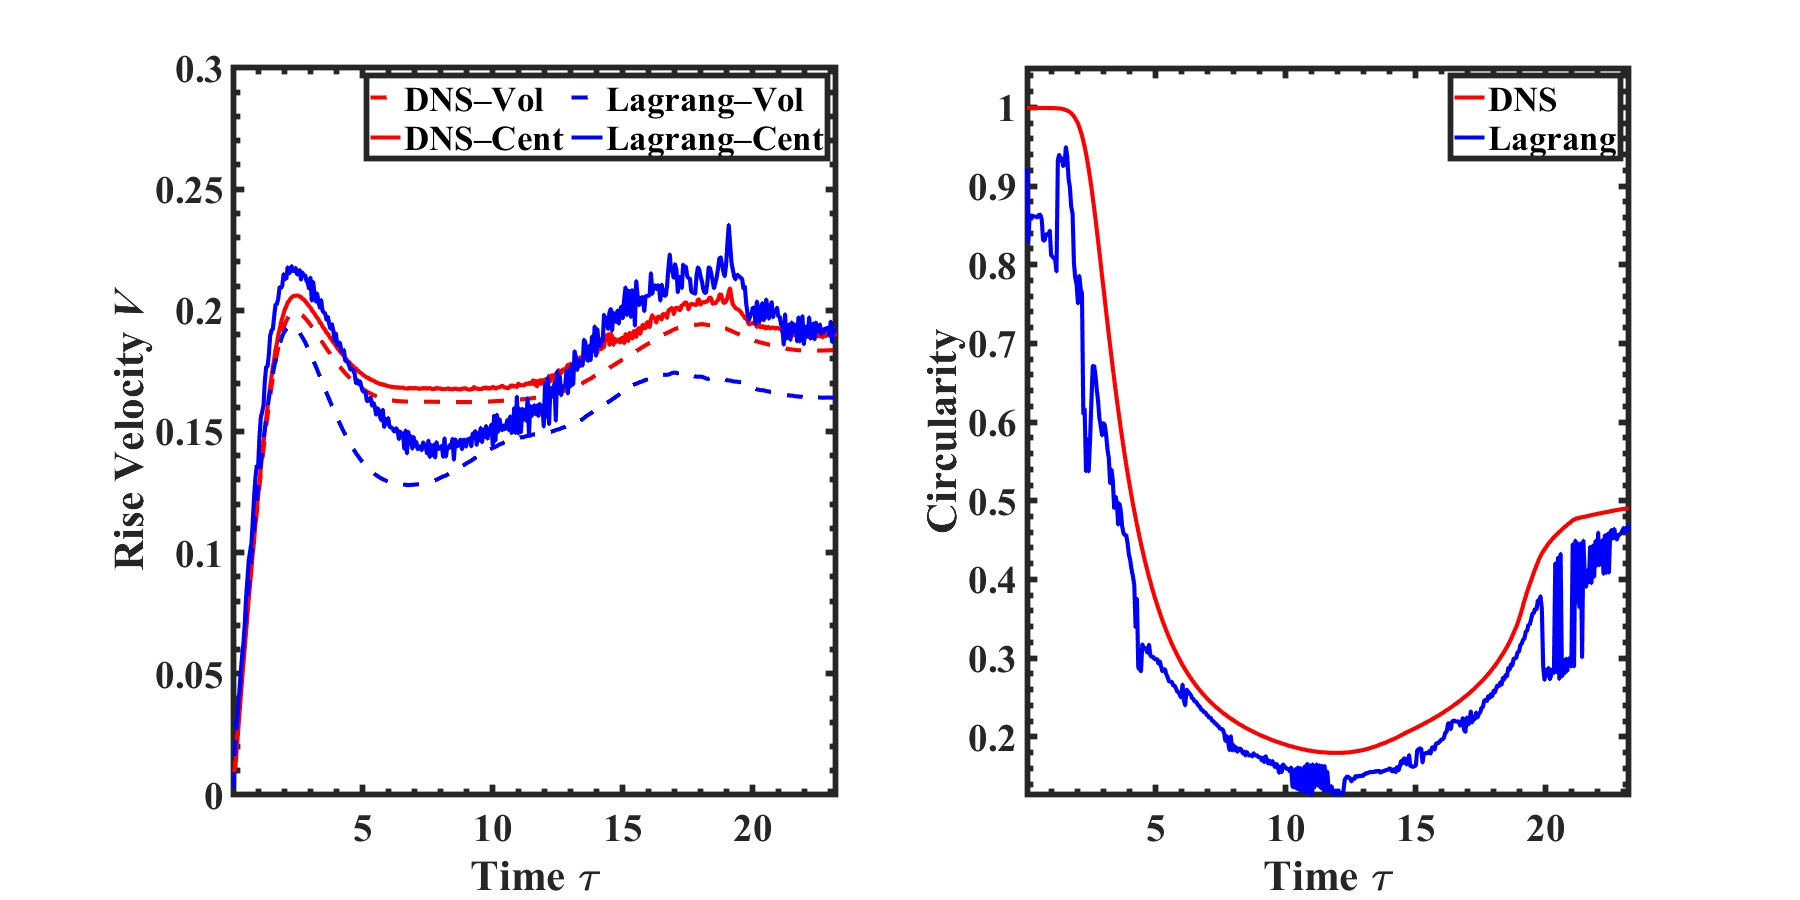
\includegraphics[width=\textwidth]{Scattered.jpg}
  \caption{Scattered Lagrangian data (Approach~A, scheme 1).
    Left: rise velocity (solid = centroid, dashed = vol-avg;
    red = Eulerian, blue = Lagrangian).
    Right: circularity.}
  \label{fig:scattered}
\end{figure}

\begin{figure}[!h]
  \centering
  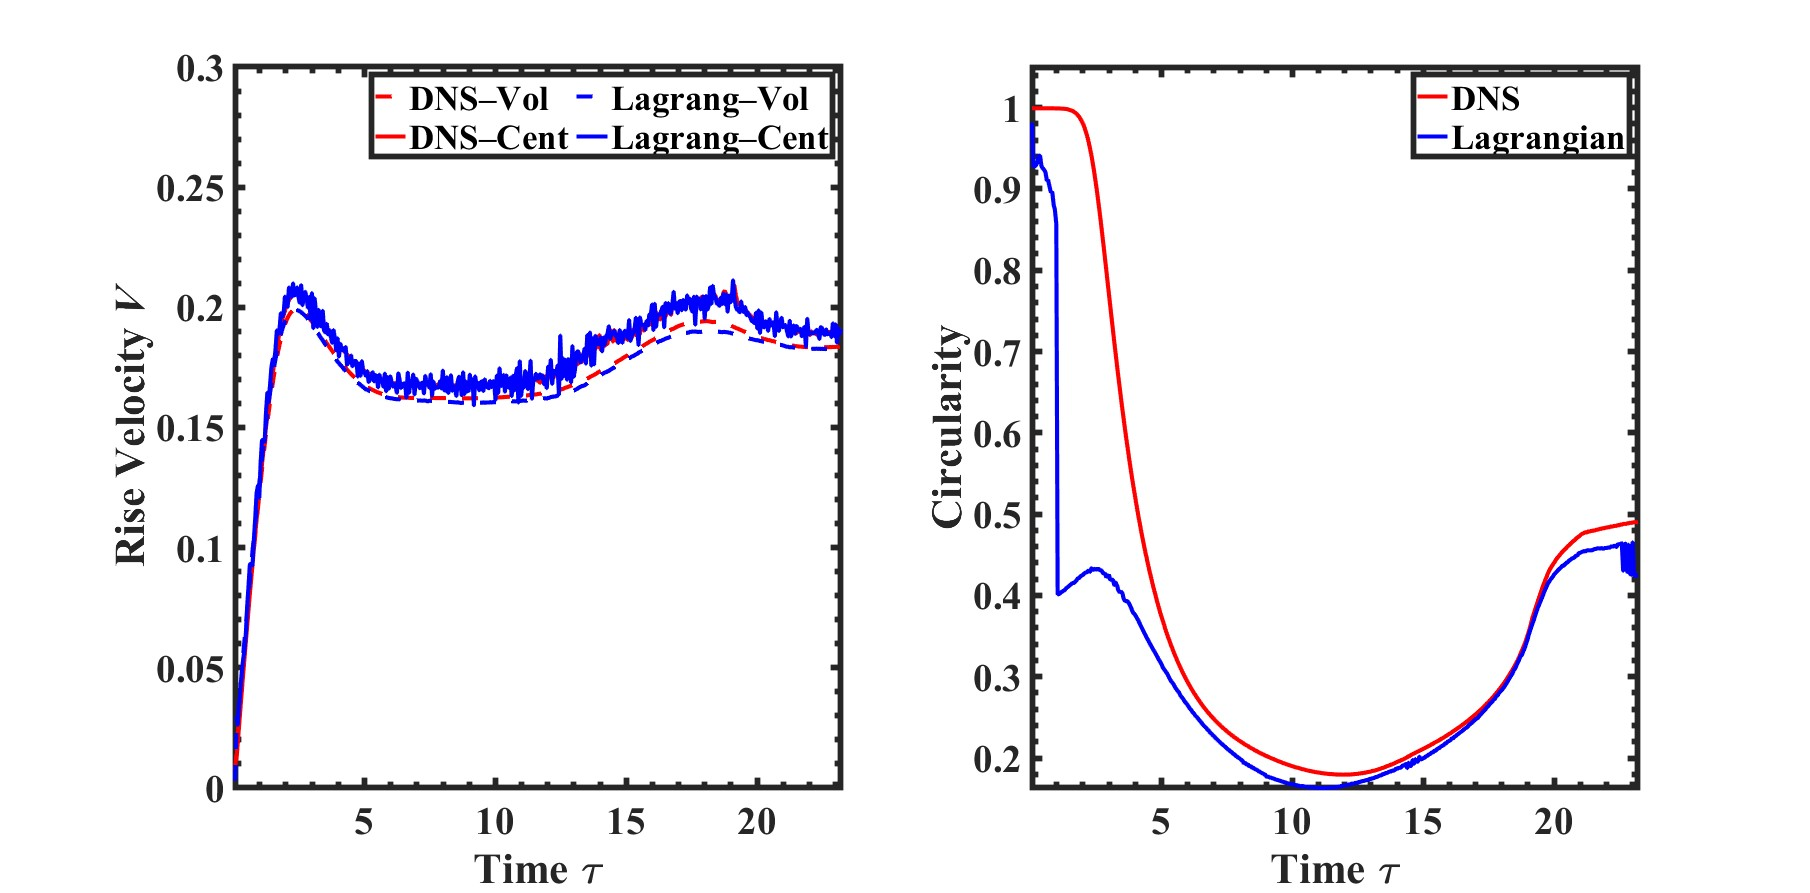
\includegraphics[width=\textwidth]{Interpolated.jpg}
  \caption{Re-interpolated Lagrangian data (Approach~B, scheme 1).
    Left: rise velocity.  Right: circularity.  Both Lagrangian curves
    (blue) now closely track the Eulerian reference (red).}
  \label{fig:interpolated}
\end{figure}


\begin{figure}[!h]
	\centering
	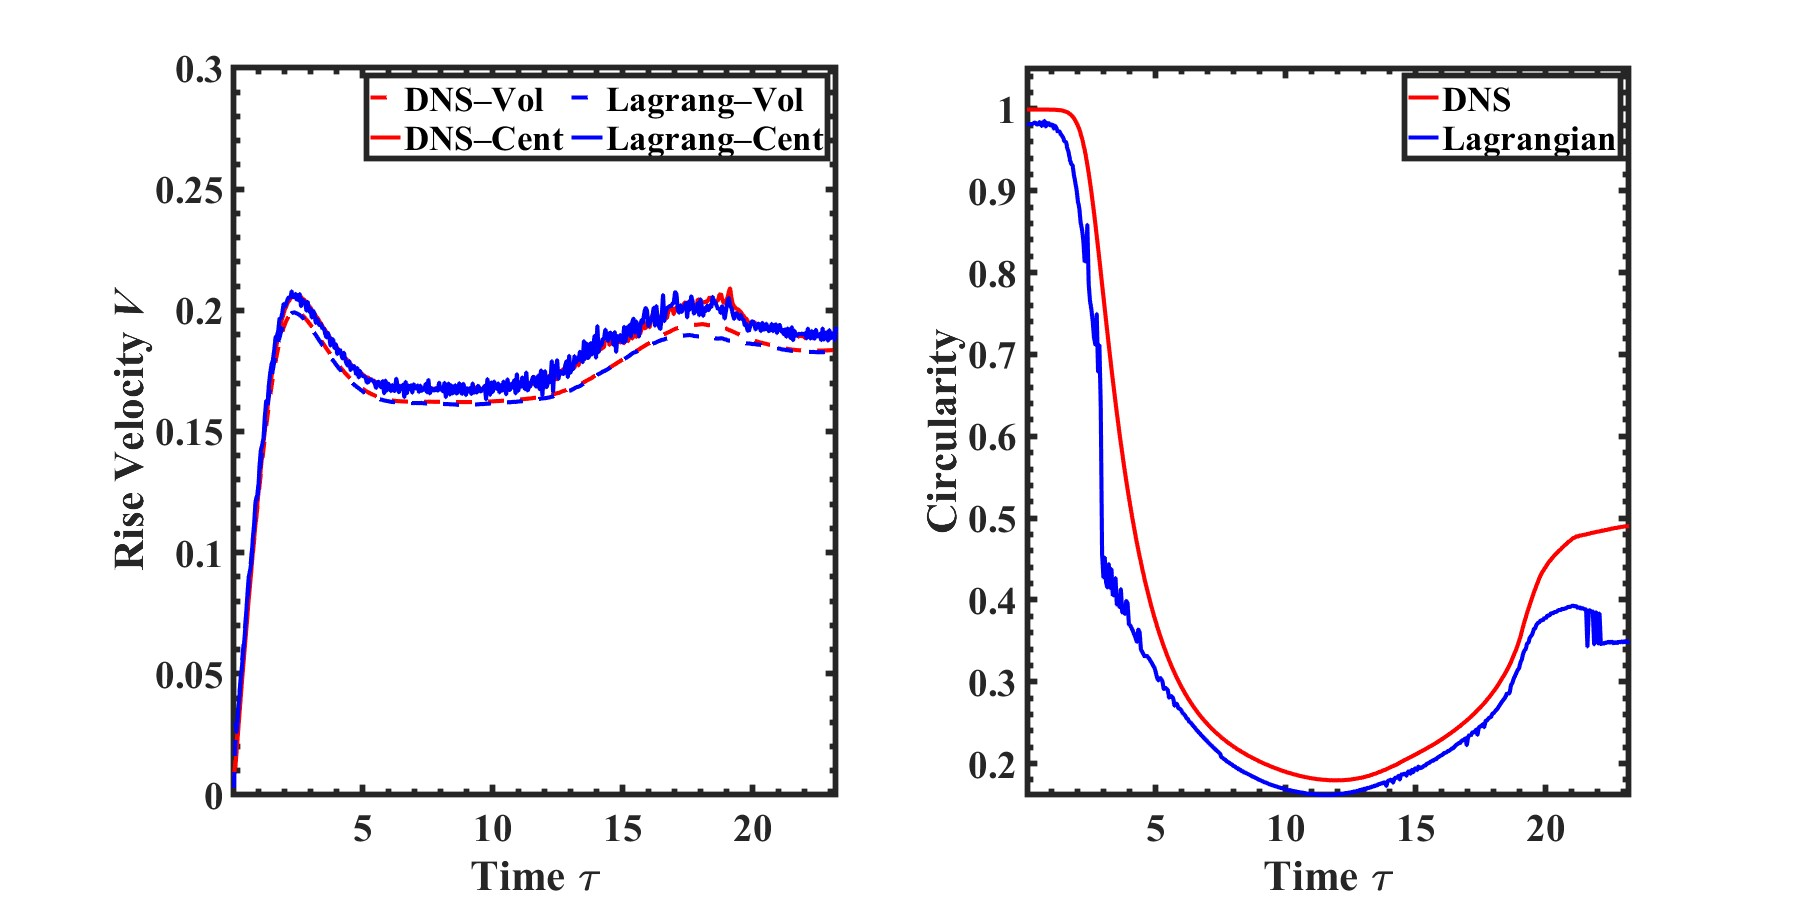
\includegraphics[width=\textwidth]{Interpolated_cubic.jpg}
	\caption{Re-interpolated Lagrangian data (Approach~B, scheme 2).
		Left: rise velocity.  Right: circularity.  Both Lagrangian curves
		(blue) now closely track the Eulerian reference (red).}
	\label{fig:interpolated_cubic_cubic}
\end{figure}

\end{document}
